\section{Auswertung}
\begin{figure}[h]
    \begin{subfigure}{0.45\textwidth}
        \centering
        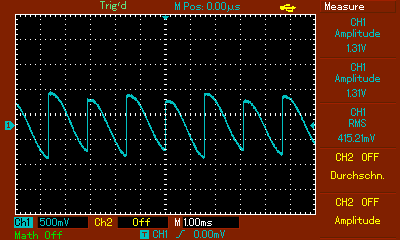
\includegraphics[width=\textwidth]{assets/0.png}
        \caption{$\phi = 0^{\circ}$}
    \end{subfigure}
    \hfill
    \begin{subfigure}{0.45\textwidth}
        \centering
        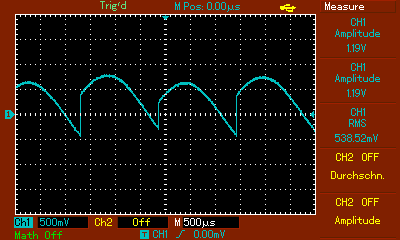
\includegraphics[width=\textwidth]{assets/45.png}
        \caption{$\phi = 45^{\circ}$}
    \end{subfigure}
    \hfill
    \begin{subfigure}{0.45\textwidth}
        \centering
        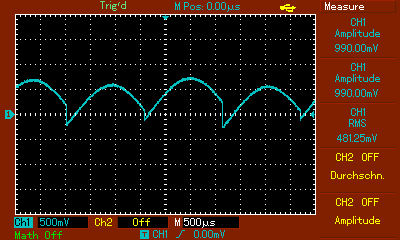
\includegraphics[width=\textwidth]{assets/90.png}
        \caption{$\phi = 90^{\circ}$}
    \end{subfigure}
    \hfill
    \begin{subfigure}{0.45\textwidth}
        \centering
        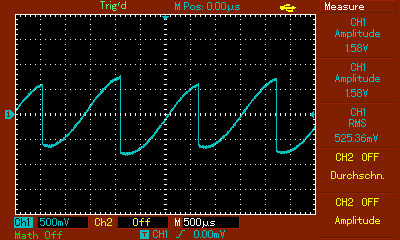
\includegraphics[width=\textwidth]{assets/180.png}
        \caption{$\phi = 180^{\circ}$}
    \end{subfigure}
    \hfill
    \begin{subfigure}{0.45\textwidth}
        \centering
        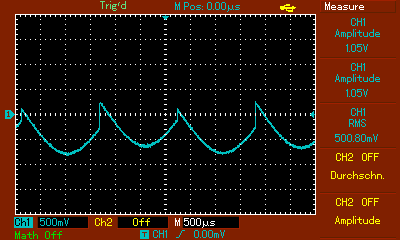
\includegraphics[width=\textwidth]{assets/270.png}
        \caption{$\phi = 270^{\circ}$}
    \end{subfigure}

    \caption{Aufgezeichnete Spannungsverläufe für das unverrauschte Signal.}
    \label{fig:unverrauscht}
\end{figure}

\begin{figure}[h]
    \begin{subfigure}{0.45\textwidth}
        \centering
        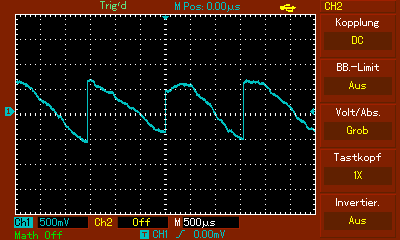
\includegraphics[width=\textwidth]{assets/0_noise.png}
        \caption{$\phi = 0^{\circ}$}
    \end{subfigure}
    \hfill
    \begin{subfigure}{0.45\textwidth}
        \centering
        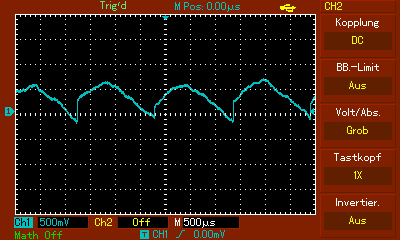
\includegraphics[width=\textwidth]{assets/45_noise.png}
        \caption{$\phi = 45^{\circ}$}
    \end{subfigure}
    \hfill
    \begin{subfigure}{0.45\textwidth}
        \centering
        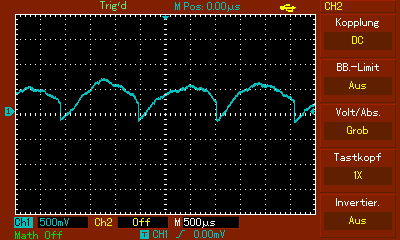
\includegraphics[width=\textwidth]{assets/90_noise.png}
        \caption{$\phi = 90^{\circ}$}
    \end{subfigure}
    \hfill
    \begin{subfigure}{0.45\textwidth}
        \centering
        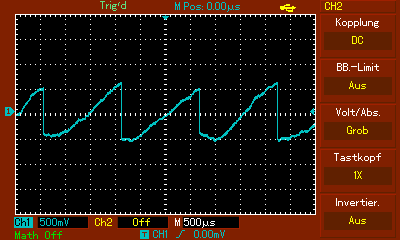
\includegraphics[width=\textwidth]{assets/180_noise.png}
        \caption{$\phi = 180^{\circ}$}
    \end{subfigure}
    \hfill
    \begin{subfigure}{0.45\textwidth}
        \centering
        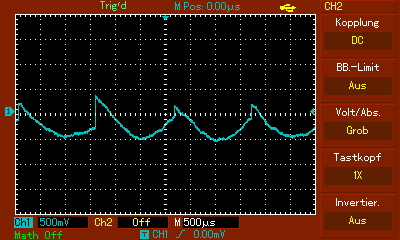
\includegraphics[width=\textwidth]{assets/270_noise.png}
        \caption{$\phi = 270^{\circ}$}
    \end{subfigure}
    \caption{Aufgezeichnete Spannungsverläufe für das verrauschte Signal.}
    \label{fig:verrauscht}
\end{figure}
\noindent In \autoref{fig:unverrauscht} sind die mit dem Oszilloskop aufgezeichneten Spannungsverläufe des unverrauschten Signals bei verschiedenen Phasenverschiebungen $\phi$ dargestellt, in \autoref{fig:verrauscht} die Spannungsverläufe des verrauschten Signales bei den selben Phasenverschiebungen. In \autoref{tab:messdaten} sind die am Tiefpass abgelesenen Spannungen bei verschiedenen $\phi$ aufgelistet. In \autoref{fig:tiefpass} sind diese Werte noch einmal graphisch dargestellt. Die Ausgleichskurven sind dabei Funktionen der Form
Die Ausgleichskurve wurde als eine Funktion der Form
\begin{equation*}
    U = a\cos{(b\phi + c)} +d .
\end{equation*}
Die Parameter wurden mit der curvefit-Funktion von Python bestimmt zu
\begin{gather*}
    a = \SI{-8.771 +- 0.240}{V} \\
    b = \num{1.008 +- 0.012} \\
    c = \num{-4.491 +- 0.047} \\
    d = \SI{-0.103 +- 0.163}{V} \\
\end{gather*}
für das unverrauschte und
\begin{gather*}
    a = \SI{-6.828 +- 0.180}{V} \\
    b = \num{1.004 +- 0.012} \\
    c = \num{-4.361 +- 0.047} \\
    d = \SI{-0.188 +- 0.125}{V} \\
\end{gather*}
für das verrauschte Signal.
\begin{table}
    \centering
    \caption{Aufgenommene Messwerte für die Ausgangsspannung am Tiefpass.}
    \label{tab:messdaten}
    \begin{tabular}{ S S S }
        \toprule
        { $\phi$ } & { $ U \: / \: \si{V} \: \text{, unverrauscht} $} & {$ U \: / \: \si{V} \: \text{, verrauscht} $} \\
        \midrule
        0          & 2.0                                              & 2.3                                           \\
        30         & 5.5                                              & 4.8                                           \\
        60         & 8.5                                              & 6.6                                           \\
        90         & 8.5                                              & 6.2                                           \\
        120        & 6.5                                              & 4.6                                           \\
        150        & 1.5                                              & 0.2                                           \\
        180        & -2.0                                             & -2.6                                          \\
        210        & -5.5                                             & -5.0                                          \\
        240        & -9.0                                             & -7.0                                          \\
        270        & -8.5                                             & -6.6                                          \\
        300        & -7.0                                             & -5.0                                          \\
        330        & -1.5                                             & -0.6                                          \\
        360        & 2.0                                              & 2.2                                           \\
    \end{tabular}
\end{table}
\begin{figure}[h]
    \begin{subfigure}{0.45\textwidth}
        \centering
        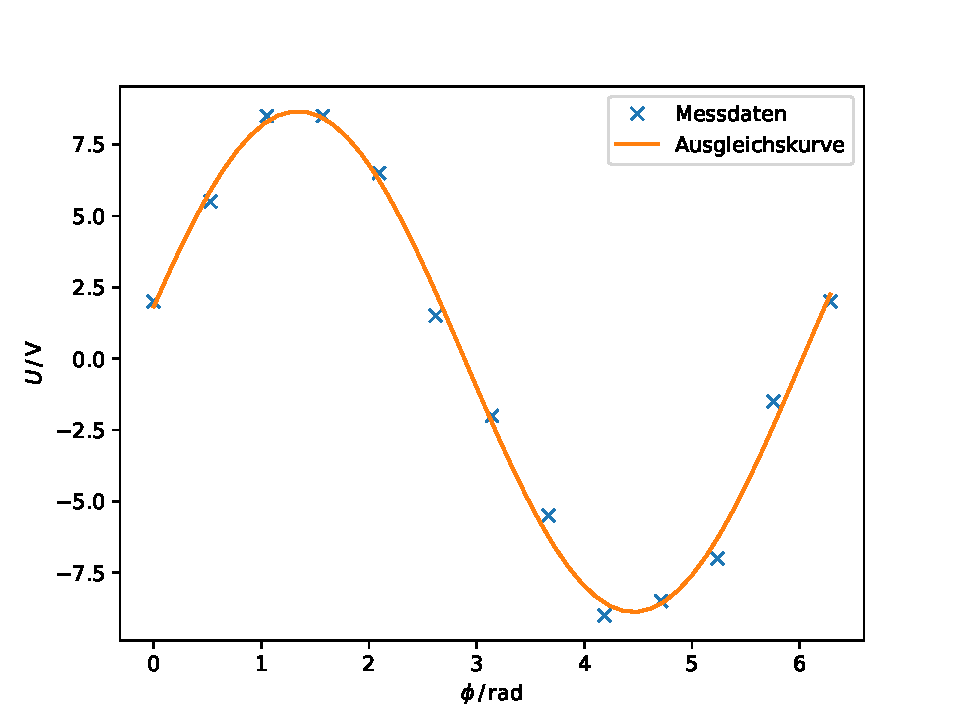
\includegraphics[width=\textwidth]{assets/plot_1.pdf}
    \end{subfigure}
    \begin{subfigure}{0.45\textwidth}
        \centering
        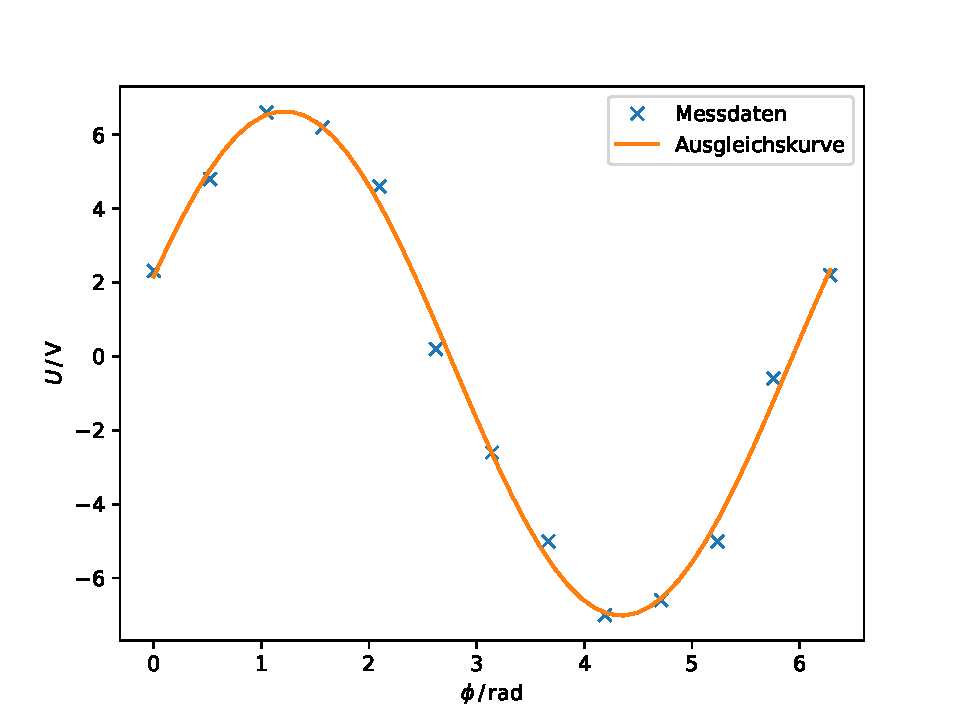
\includegraphics[width=\textwidth]{assets/plot_2.pdf}
    \end{subfigure}
    \caption{Messdaten für die Ausgangsspannung am Tiefpass}
    \label{fig:tiefpass}
\end{figure}

\noindent In \autoref{tab:messdaten_LED} sind die aufgenommenen Werte für die gemessene Ausgangsspannung bei verschiedenen Abständen zwischen der LED und der Photodiode aufgelistet, in \autoref{fig:LED} sind diese dazu einmal einfach gegen $r$ und einmal doppelt logarithmisch aufgetragen.
\begin{table}
    \centering
    \caption{Aufgenommene Messwerte für die Spannung in Abhängigkeit vom Abstand.}
    \label{tab:messdaten_LED}
    \begin{tabular}{ S S }
        \toprule
        {  $ r \: / \: \si{cm} $ } & { $ U \: / \: \si{V} $} \\
        \midrule
        5                          & 8.00                    \\
        10                         & 4.50                    \\
        15                         & 2.00                    \\
        20                         & 1.50                    \\
        25                         & 0.65                    \\
        30                         & 0.45                    \\
        35                         & 0.35                    \\
        40                         & 0.25                    \\
        45                         & 0.20                    \\
        55                         & 0.15                    \\
        65                         & 0.10                    \\
        90                         & 0.05                    \\
        146                        & 0.05                    \\
    \end{tabular}
\end{table}
\begin{figure}[h]
    \begin{subfigure}{0.45\textwidth}
        \centering
        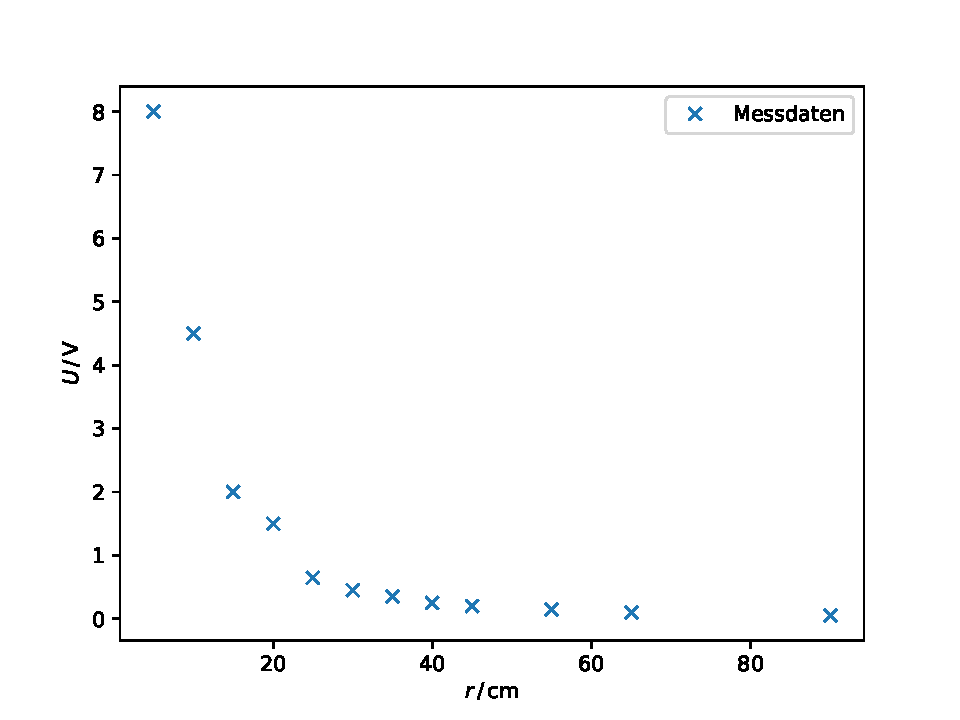
\includegraphics[width=\textwidth]{assets/plot_3.pdf}
    \end{subfigure}
    \begin{subfigure}{0.45\textwidth}
        \centering
        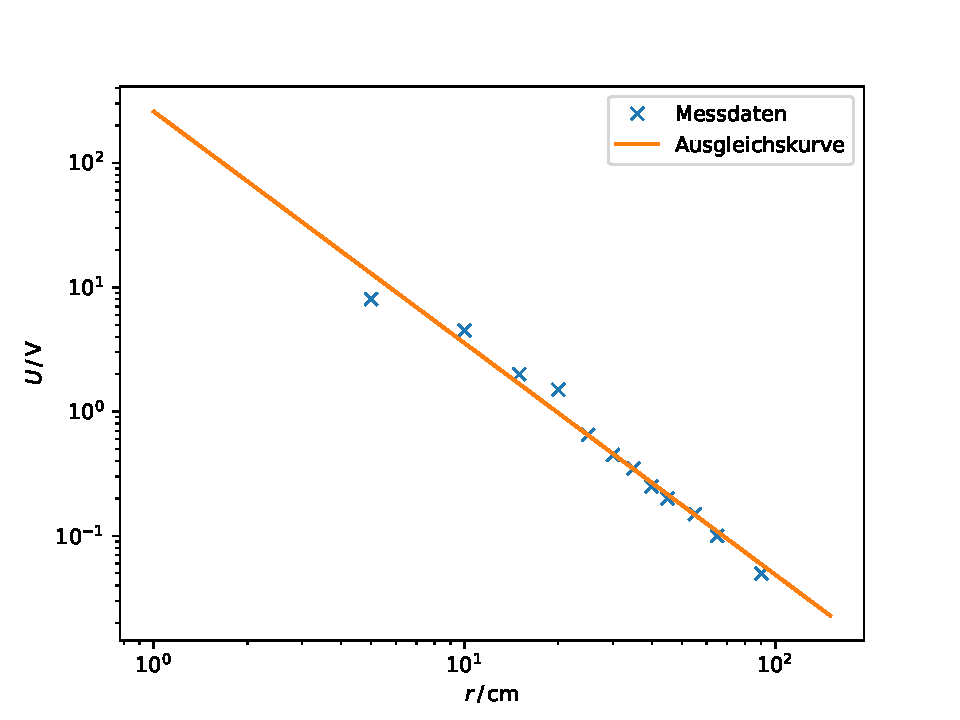
\includegraphics[width=\textwidth]{assets/plot_4.pdf}
    \end{subfigure}
    \caption{Gemessene Spannung in Abhängigkeit vom Abstand.}
    \label{fig:LED}
\end{figure}
Da beim letzten aufgenommenen Messwert trotz des großen Schrittes für $r$ keine Änderung mehr für $U$ abzulesen war, kann davon ausgegangen werden, dass an diesem Punkt nur noch die Raumbeleuchtung von der Photodiode aufgenommen wurde und nicht mehr das Signal der LED. Bei der Ausgleichrechnung wurde dieser Messpunkt daher nicht mehr beachtet. In der logarithmischen Darstellung ist zu sehen, dass alle Messpunkte annähernd auf einer Geraden liegen. Die berechnete Ausgleichsgerade hat die Form
\begin{align*}
                     & \log{U} & = k \cdot \log{r} + \log{C} \\
    \text{mit} \quad & k       & = \num{-1.862 +- 0.086} \:, \\
                     & \log{C} & = \num{5.554 +- 0.294} .
\end{align*}
Durch exponenzieren der Geradengleichung erhält man eine Funktion der Form
\begin{align*}
             & U = C \cdot r^k \\
    \implies & U \propto r^k
\end{align*}